\section{Global}
In each calculation of the global sensitivity analysis, we varied 
the transition start 
time, percent of \glspl{LWR} operating for 80 years, the Xe-100 discharge 
burnup, \gls{MMR} burnup, and build share of one advanced reactor. 
We decided to perform this analysis three separate times instead of 
varying all seven variables to prevent unwanted combinations of the 
advanced reactor build shares that result in an oversupply or 
undersupply of power. 

Instead of comparing ranges and values of each metric in this 
analysis, we compared the variance each input parameter causes in 
the output metrics through the Sobol' indices. 
To assist in calculating the Sobol' indices, we created surrogate 
models for each of the iterations. These models are approximations 
of the relationships between the input and output parameters,
are computationally inexpensive \cite{adams_dakota_2021}, and 
assist in exploring an entire input space, as compared with 
exploring an input space in a grid search. To generate 
each of the surrogate models (one for each advanced reactor build share 
variation), we ran 4000 different fuel cycle transitions based on guidance 
from the Dakota manual \cite{adams_dakota_2021} to run 

\begin{equation}
    100\times P\times(R+2)
    \label{eq:surrogate}
\end{equation}

\noindent number of cases to build the surrogate model 
In Eq \ref{eq:surrogate}, $P$ is the number of input parameters and 
$R$ is the number out response metrics. 

In each of these
transitions, we allowed most of the input parameters vary freely 
within a given range (defined in Table \ref{tab:global_ranges}), 
and used Latin Hypercube Sampling (a near-random technique in 
Dakota) to select parameter values. We did not allow 
the Xe-100 discharge burnup to vary freely within a range 
when running the initial transition scenarios. We kept this input
parameter constrained to 
specific values, like in the \gls{OAT} analysis. The burnup values 
considered for the sensitivity 
analysis thus far are based on integer numbers of passes through 
the core (batches) and integer number of 
months for the cycle lengths of this reactor. By using 
Xe-100 burnup values that correspond to integer values, we can 
adhere to the integer value restrictions in \Cyclus on the number of 
batches in a core.
We expanded the Xe-100 discharge burnup values considered 
to provide additional data points off of which to 
generate the surrogate model. We selected additional burnup points 
to represent 
between one and six passes for each pebble with a residence time of six, seven, 
or eight months for each pass. This expansion of the Xe-100 burnup resulted 
in 16 different burnup values between 28-185 MWd/kgU.
We converted the \gls{MMR} burnup 
from a discrete variable to a continuous variable by varying 
the lifetime of the reactor as need to achieve the burnup value. We made 
this conversion from discrete to continuous for the \gls{MMR} burnup 
because the lack of multiple batches in the core means that there are 
no inherent restrictions to integer numbers. 

\begin{table}[h!]
    \centering 
    \caption{Ranges of the input parameters considered for generating 
    surrogate models in the global sensitivity analysis. The Xe-100 
    burnup was constrained to 16 different values within the given range, 
    while the other variables were free to vary within the defined range.}
    \label{tab:global_ranges}
    \begin{tabular}{c c c}
        \hline
        Input parameter & Range & Units \\
        \hline 
        Transition start time & January 2025-January 2040 & - \\
        LWR lifetime extensions & 0-50 & \% \\
        Reactor build share & 0-50 & \% \\
        \gls{MMR} burnup & 41-90 & MWd/kg \\
        Xe-100 burnup & 28-185 & MWd/kg \\
        \hline
    \end{tabular}
\end{table}

After explicitly modeling the transition scenarios with different 
combinations and the specific Xe-100 burnup values, we 
created surrogate models. 
When creating the surrogate model, we once again used the Latin Hypercube 
sampling 
for all of the variables, but allowed all of the input parameters to be 
continuous variables. The surrogate models are not bound by 
the variable-type restriction in \Cyclus, so we were able to allow 
the Xe-100 burnup to not be bound by integer numbers of batches. 
We used both the quadratic and Gaussian fits to the data 
to create the surrogate models, similar to what Richards and 
Feng did \cite{richards_application_2021}. The quadratic method defines a 
second-order response surface based on linear least squares regressions methods 
\cite{adams_dakota_2021}. The Gaussian method uses a Gaussian correlation function 
to define a response surface \cite{adams_dakota_2021}. We used both methods were 
used to provide a comparison of the different methods, since they each have
limitations. 
The quadratic method does not implement any forward- or backward-stepping regression 
methods to remove unnecessary terms in the polynomial fit, and the Gaussian method 
may discard points if the data points are poorly spaced \cite{adams_dakota_2021}.
These limitations in the methods contributed to the decision to have as many 
input parameter data points as possible. 
We also instructed Dakota to perform variance decomposition 
on both of the surrogate models to calculate the Sobol' indices.

The results presented in this section include the results from the initial 
transitions modeled, the results from the surrogate models, and the Sobol' indices 
that describes the impact of each input parameter on each output metric. The 
results from the modeled transitions and the surrogate models provide 
information of how well the surrogate models fit some of the trends and 
relationships 
between the input parameters and output metrics. 
The total and the main Sobol' indices reported describe the contribution 
from each parameter and its interactions with all of the other parameters 
and the contribution from each individual parameter, respectively. 

\subsection{Xe-100 build share}
This section provides the results of the global sensitivity analysis using 
both a Gaussian and a quadratic surrogate model when varying the Xe-100 build 
share. 

\subsubsection{Gaussian surrogate model}
The Gaussian surrogate model for the variations in the Xe-100 build 
share results in an R$^2$ value of 1 for each metric. This value 
means that the outputs of 
the surrogate model match perfectly to the data provided from the initial 
\Cyclus runs. The large R$^2$ value suggests that this surrogate model type 
fits to noise in the data provided. 
Figure \ref{fig:s7_xe100_gaussian} compares the values of the
\gls{HALEU} mass as a function of the Xe-100 burnup for the Gaussian model 
and the input data (the explicitly modeled transitions). The results of 
the Gaussian model follows the input 
data well, nearly reaching the maximum and minimums of the data. However, 
closer inspection of the data shows that results of the Gaussian model 
include non-physical results, such as negative values of \gls{HALEU} mass. 
These values suggest that the Gaussian model extrapolates to obtain 
some of the values, instead 
of just interpolating. Therefore, the Gaussian model is not a perfect 
match to the input data, which means that the Sobol' indices are different 
than if the variance decomposition were performed directly on the input 
data. 

\begin{figure}[h!]
    \centering 
    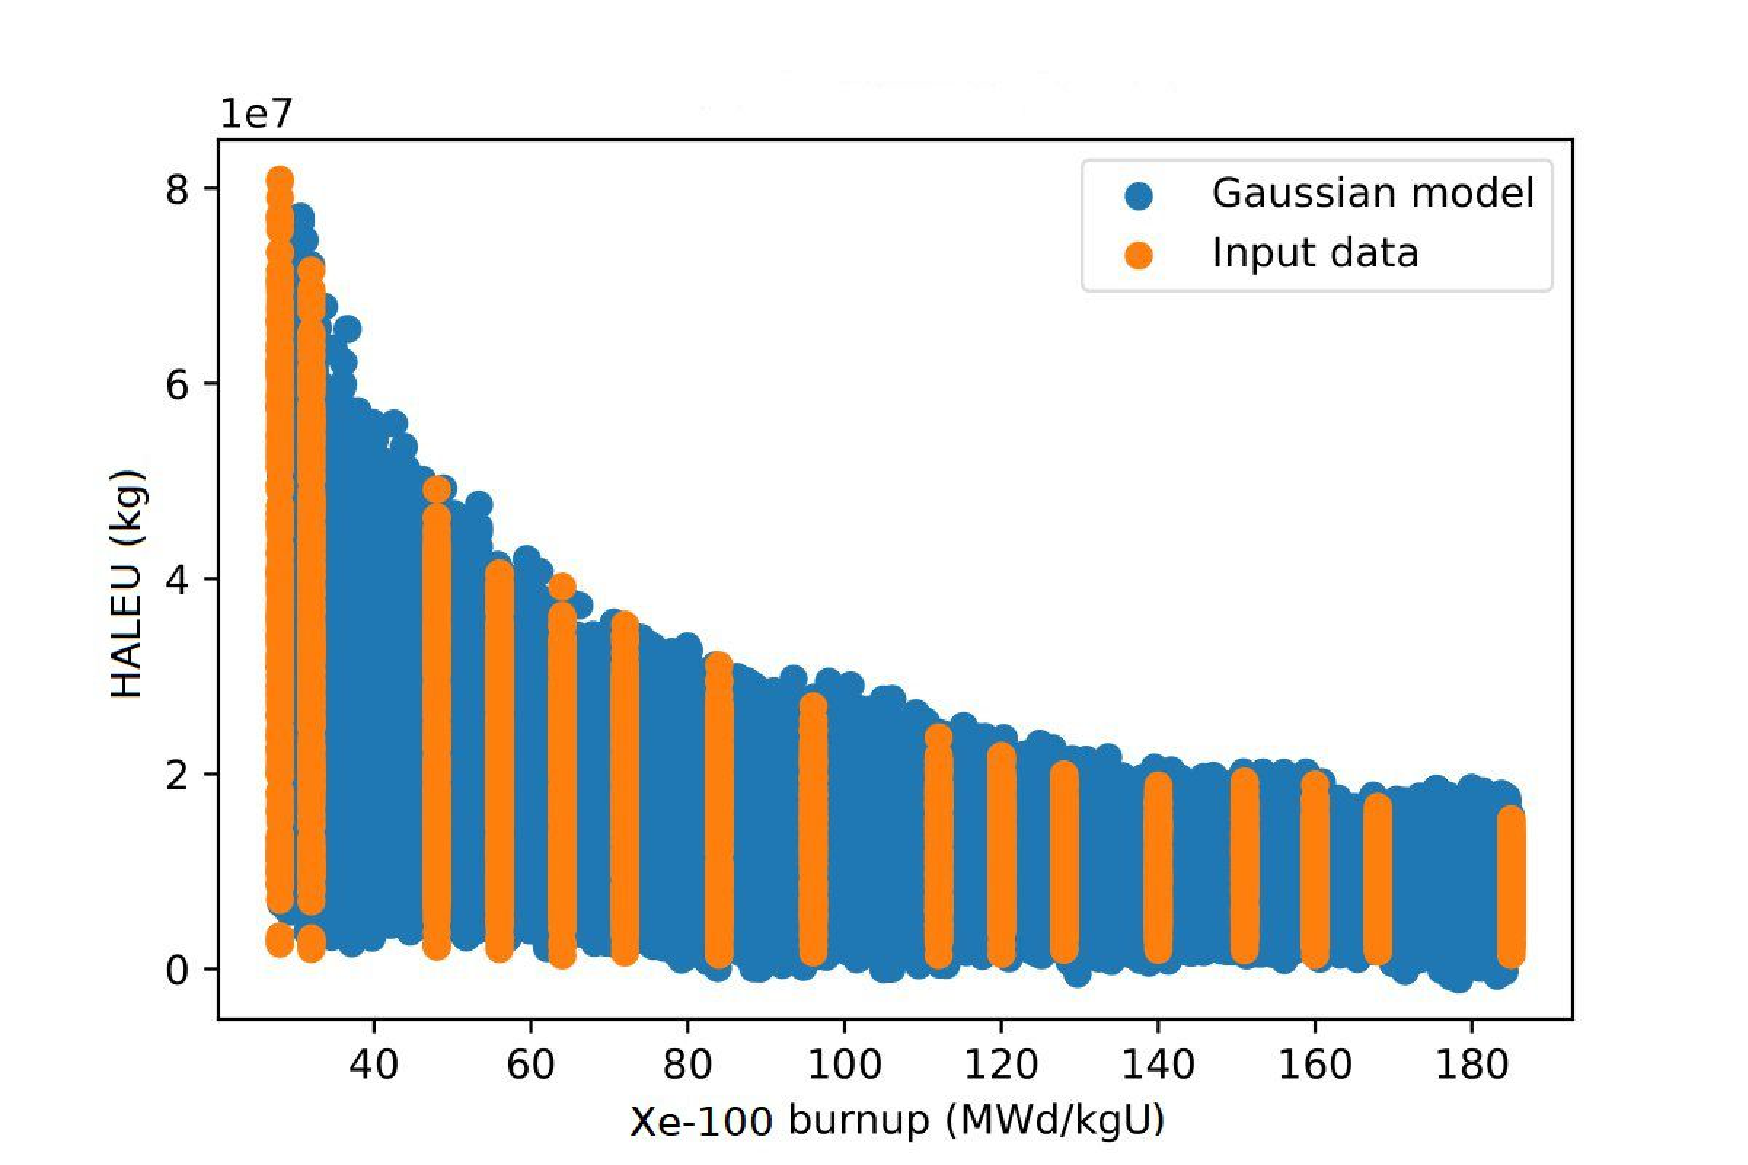
\includegraphics[scale=0.8]{xe100_share_gaussian_xe100_burnup_haleu.pdf}
    \caption{Comparison of the input data and the results of the Gaussian 
    surrogate model when the Xe-100 build share is varied.}
    \label{fig:s7_xe100_gaussian}
\end{figure}

Table \ref{tab:s7_sobol_xe100_gaussian} reports the main and total Sobol' indices 
for each input parameter on each output metric. The highlighted cells have 
a total Sobol' index of at least 0.5, to indicate parameters that have a large 
effect on the metrics. 
The transition start time 
has little effect on any of the metrics, which is consistent with the 
results of the \gls{OAT} and synergistic analysis. The \gls{LWR} lifetimes 
do not greatly affect any of the \gls{HALEU}-related metrics or the 
total \gls{SWU} capacity because this parameter primarily delays when 
the \gls{HALEU}-fueled reactors are deployed and not how many are deployed. 
The \gls{LWR} lifetimes have some impact on the total 
fuel mass and the \gls{SNF} mass, but less of an impact than the Xe-100 
build share. 
The \gls{MMR} burnup has a small Sobol' index for all of the output metrics
because a very small portion of the fleet are \glspl{MMR}. 

The Xe-100 build share and burnup have a large effect (total Sobol' indices 
more than 0.5) on all three of the \gls{HALEU}-related metrics because the 
number of \glspl{MMR} built in these transitions are relatively constant and the 
variations in the Xe-100s drive the changes in these metrics. The Xe-100 build share 
does not have as much of an impact on the total \gls{SWU} capacity because 
of the similar \gls{SWU} capacity required by the Xe-100 and the VOYGR and 
the replacement of VOYGRs with Xe-100s as the Xe-100 build share increases. 
The Xe-100 build share has the largest impact on the total fuel mass 
and the \gls{SNF} mass because 
of the replacement of Xe-100s with VOYGRs as the Xe-100 build share decreases and 
the large difference in fuel mass required by these two reactors. The Xe-100 
burnup has the largest impact on the total \gls{SWU} capacity because as this 
parameter varies, so does the difference in \gls{SWU} capacity needed to fuel the Xe-100 
and the \gls{SWU} capacity needed to fuel the VOYGR.

\begin{table}[h!]
    \centering
    \caption{Sobol' indices for the Gaussian model when varying the 
    Xe-100 build share. The first value is the 
    main index, the second value is the total index. Highlighted 
    values indicate a total Sobol' indices of above 0.5.}
    \label{tab:s7_sobol_xe100_gaussian}
    \begin{tabular}{c c c c c c c}
        \hline
        & \multicolumn{6}{c}{Output Metric} \\
        Parameter & Fuel Mass & HALEU Mass & SWU & HALEU SWU & Feed & SNF Mass \\
        \hline
        Transition Start & 0.003/0.003 & 0.007/0.007 & 0.007/0.009 &
                           0.009/0.009 & 0.006/0.009 & 0.003/0.003\\
        LWR Lifetime & 0.268/0.280 & 0.012/0.021 & 0.081/0.095 &
                       0.013/0.022 & 0.013/0.022 & 0.301/0.314\\
        Xe-100 Build Share & \cellcolor{green!25}0.478/0.533 & \cellcolor{green!25}0.375/0.513 & 0.099/0.283 &
        \cellcolor{green!25}0.374/0.511 & \cellcolor{green!25}0.374/0.512 & 0.411/0.474\\
        Xe-100 Burnup & 0.188/0.247 & \cellcolor{green!25}0.465/0.571 & \cellcolor{green!25}0.622/0.775 & 
        \cellcolor{green!25}0.463/0.568 & \cellcolor{green!25}0.463/0.568 & 0.214/0.280\\
        MMR Burnup & 0.002/0.002 & 0.003/0.004 & 0.005/0.006 & 
                     0.004/0.005 & 0.004/0.005 & 0.002/0.002\\
        \hline        
    \end{tabular}
\end{table}

\subsubsection{Quadratic surrogate model}
When using a quadratic surrogate model, the R$^2$ values for the training points on 
each output metric range between 0.921-0.966. Therefore, these model are  
expected to 
fit the input data provided but not be fit to the noise in the input data 
as much as the Gaussian model. A comparison of the Xe-100 burnup and \gls{HALEU} 
mass for the input data and the results of the quadratic model (Figure 
\ref{fig:s7_xe100_quadratic}) shows that the quadratic model does 
capture the overall trend of the input data. However, like the Gaussian model, 
the quadratic model gives the non-physical result of a negative \gls{HALEU} mass
at some points. Additionally, 
the results of the quadratic model do not meet the maximum of the input data and 
provide multiple results below the minimum value of the input data. Therefore, 
the quadratic model is also performing some extrapolation of the data based on the 
fit placed on the data.

\begin{figure}[h!]
    \centering 
    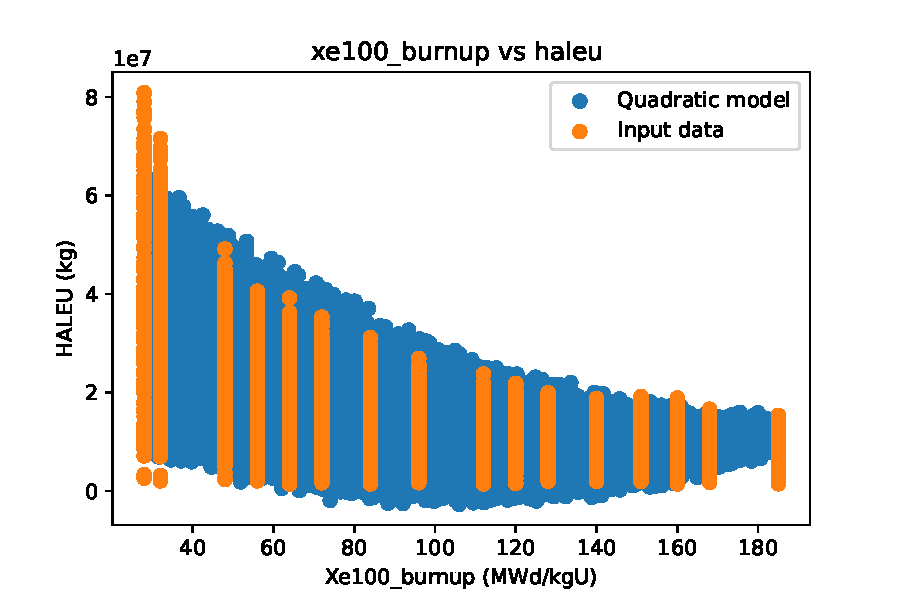
\includegraphics[scale=0.8]{xe100_share_quadratic_xe100_burnup_haleu.pdf}
    \caption{Comparison of the input data and the results of the quadratic 
    surrogate model when the Xe-100 build share is varied.}
    \label{fig:s7_xe100_quadratic}
\end{figure}

Table \ref{tab:s7_sobol_xe100_quadratic} provides the main and total Sobol' 
indices for each of the input parameters on each output metric. The 
green cells identify total Sobol' indices that are at least 0.5. The same patterns 
observed in the Sobol' indices from the Gaussian model are 
observed in the values from the quadratic model as well. The Xe-100 build share 
and Xe-100 burnup affect the metrics the most, the \gls{LWR} lifetime has some 
impact, and the \gls{MMR} burnup and transition start time has the smallest impact 
on the metrics. 

\begin{table}[h!]
    \centering
    \caption{Sobol' indices for the quadratic model when varying the Xe-100 
    build share. The first number is the main index, the second is the total 
    index. Highlighted 
    values indicate a total Sobol' indices of above 0.5.}
    \label{tab:s7_sobol_xe100_quadratic}
    \begin{tabular}{c c c c c c c}
        \hline
        & \multicolumn{6}{c}{Output Metric} \\
        Parameter & Fuel Mass & HALEU Mass & SWU & HALEU SWU & Feed & SNF Mass \\
        \hline
        Transition Start & 0.000/0.000& 0.006/0.005 & 0.007/0.007 &
                           0.008/0.007 & 0.008/0.007 & 0.002/0.004\\
        LWR Lifetime & 0.278/0.286 & 0.014/0.021 & 0.082/0.089 & 
                       0.015/0.022 & 0.015/0.022 & 0.310/0.319\\
        Xe-100 Build Share & \cellcolor{green!25}0.443/0.501 & \cellcolor{green!25}0.374/0.500 & 0.115/0.283 & 
                             0.374/0.499 & 0.374/0.499 & 0.375/0.441\\
        Xe-100 Burnup & 0.214/0.279 & \cellcolor{green!25}0.472/0.578 & \cellcolor{green!25}0.624/0.773 &
                        \cellcolor{green!25}0.470/0.576 & \cellcolor{green!25}0.430/0.576 & 0.243/0.315\\
        MMR Burnup & 0.001/0.001 & 0.002/0.002 & 0.004/0.004 &
                     0.003/0.003 & 0.003/0.003 & 0.001/0.001\\
        \hline        
    \end{tabular}
\end{table}

The two surrogate models result in different Sobol' indices for each 
input parameter/output metric pair. These differences are likely a result 
of how the models fit the data. The Gaussian model fits 
better the the extremes and trends in the input data points, but the 
quadratic model does fit to the noise in the input data as much. 
However, the two models are consistent in 
their relative comparison of how much each input parameter affects the output 
metrics, and are consistent with the results from the \gls{OAT} and 
synergistic analysis. The two models are also consistent in 
identifying that the Xe-100 build share and Xe-100 burnup 
have the largest impact on the metrics.

\subsection{MMR build share}
This section provides the results of the global sensitivity analysis using 
both a Gaussian and a quadratic surrogate model when varying the \gls{MMR} 
build share. 

\subsubsection{Gaussian surrogate model}
The Gaussian model has an R$^2$ value of 1 with respect to each of the output 
metrics. This value means that these models are also expected to fit the input 
data very well, including any noise present in the data. As Figure 
\ref{fig:s7_mmr_gaussian} shows, the data from the Gaussian model fits well 
to the input data provided. Unlike the models predicted based on input data when 
varying the Xe-100 build share, this model does not result in any negative 
mass values. However, it still results in mass values lower than what is 
present in the input data which suggests that this model also extrapolates 
on some of the data. It also does not fully predict some of the outliers in 
the data, such as the maximum \gls{HALEU} mass at a burnup at 128 MWd/kg.

\begin{figure}[h!]
    \centering 
    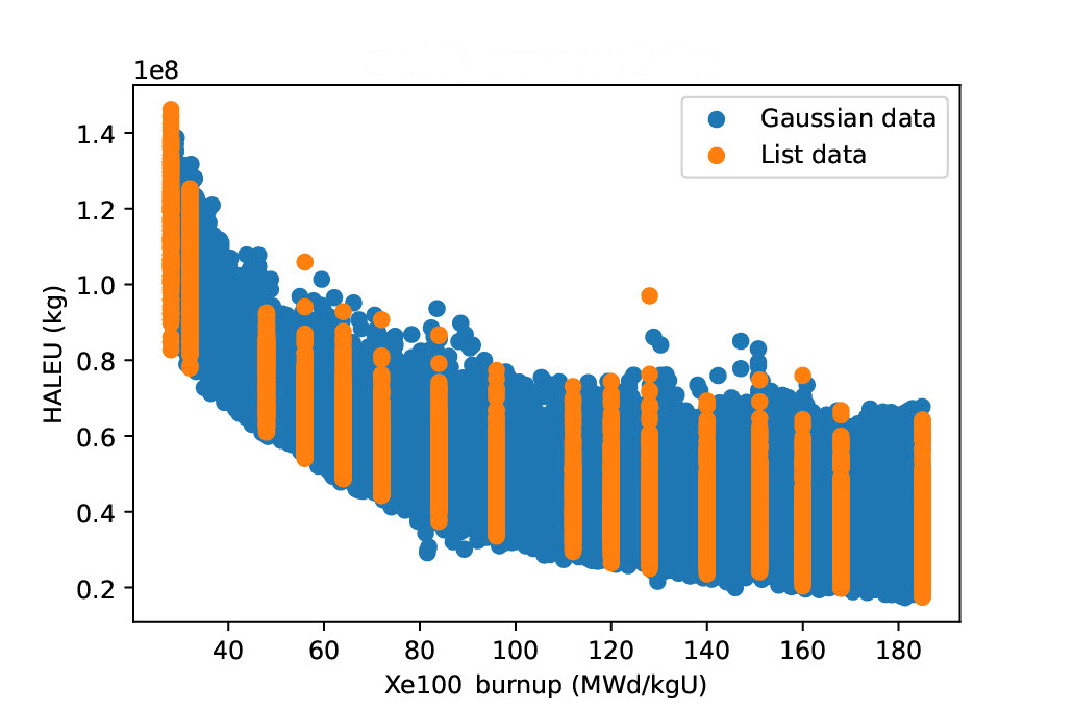
\includegraphics[scale=0.8]{mmr_share_gaussian_xe100_burnup_haleu.pdf}
    \caption{Comparison of the input data and the results of the Gaussian 
    surrogate model when varying the MMR build share.}
    \label{fig:s7_mmr_gaussian}
\end{figure}

Examination of the Sobol' indices for this model (Table \ref{tab:s7_sobol_mmr_gaussian})
shows that the Xe-100 burnup has the largest impact and a significant impact (i.e., 
total indices greater than 0.5) on all of the 
output metrics. One may expect the \gls{MMR} 
build share and \gls{MMR} burnup to have a strong combined impact on 
the results. However, this result is consistent with the results 
shown for the synergistic analysis (Figures \ref{fig:mmr_share_xe100_burnup} and 
\ref{fig:mmr_share_mmr_burnup}). When the Xe-100 burnup was varied in combination 
with the \gls{MMR} share, the range of values for each metric was larger than 
when the \gls{MMR} burnup was varied with the \gls{MMR} build share. Variations 
in the \gls{MMR} build share replaces Xe-100s with \glspl{MMR}. The variations 
in the Xe-100 burnup lead to greater changes in the metrics than variations 
in the \gls{MMR} burnup, as shown in Figure \ref{fig:bu_constant}, because 
the Xe-100 burnup values span a larger range and the compounding effects of the 
multiple batches in the Xe-100. 
Similar to the results from varying the Xe-100 build share, the 
transition start time has effectively no impact on the results. The \gls{LWR} 
lifetime has less of an impact on the metrics than when the Xe-100 
build share was varied. The \gls{MMR} burnup also has little impact on the 
output metrics. 

\begin{table}[h!]
    \centering
    \caption{Sobol' indices for the Gaussian model when varying the MMR 
    build share. The first number is the main index, the second is the total 
    index. Highlighted 
    values indicate a total Sobol' indices of above 0.5.}
    \label{tab:s7_sobol_mmr_gaussian}
    \begin{tabular}{c c c c c c c}
        \hline
        & \multicolumn{6}{c}{Output Metric} \\
        Parameter & Fuel Mass & HALEU Mass & SWU & HALEU SWU & Feed & SNF Mass \\
        \hline
        Transition Start & 0.001/0.006 & 0.000/0.004 & 0.001/0.001 &
                           0.001/0.001 & 0.001/0.001 & 0.001/0.006\\
        LWR Lifetime & 0.054/0.068 & 0.047/0.063 & 0.055/0.071 &
                       0.054/0.069 & 0.054/0.069 & 0.057/0.071\\
        MMR Build Share & 0.069/0.107 & 0.068/0.107 & 0.162/0.203 &
                          0.162/0.204 & 0.152/0.193 & 0.015/0.055\\
        Xe-100 Burnup & \cellcolor{green!25}0.806/0.846 & \cellcolor{green!25}0.819/0.858 & \cellcolor{green!25}0.700/0.732 &
        \cellcolor{green!25}0.701/0.734 & \cellcolor{green!25}0.713/0.747 & \cellcolor{green!25}0.858/0.900\\
        MMR Burnup & 0.035/0.049 & 0.037/0.050 & 0.054/0.071 &
                     0.054/0.071 & 0.052/0.069 & 0.038/0.053\\
        \hline        
    \end{tabular}
\end{table}

\subsubsection{Quadratic surrogate model}
When using the quadratic surrogate model, the model has an R$^2$ value of 0.94
with respect to each of the output metrics. Therefore, these models also fit 
the data well without fitting all of the noise present in the input data. 
As Figure \ref{fig:s7_mmr_quadratic} shows, the output of the quadratic model 
fits the input data well, but not perfectly. Similar to the quadratic 
model created from varying the Xe-100 build share, this model 
does not perform well in fitting the maximum values and under-predicts 
some of the minimum values in the input data. 

\begin{figure}[h!]
    \centering 
    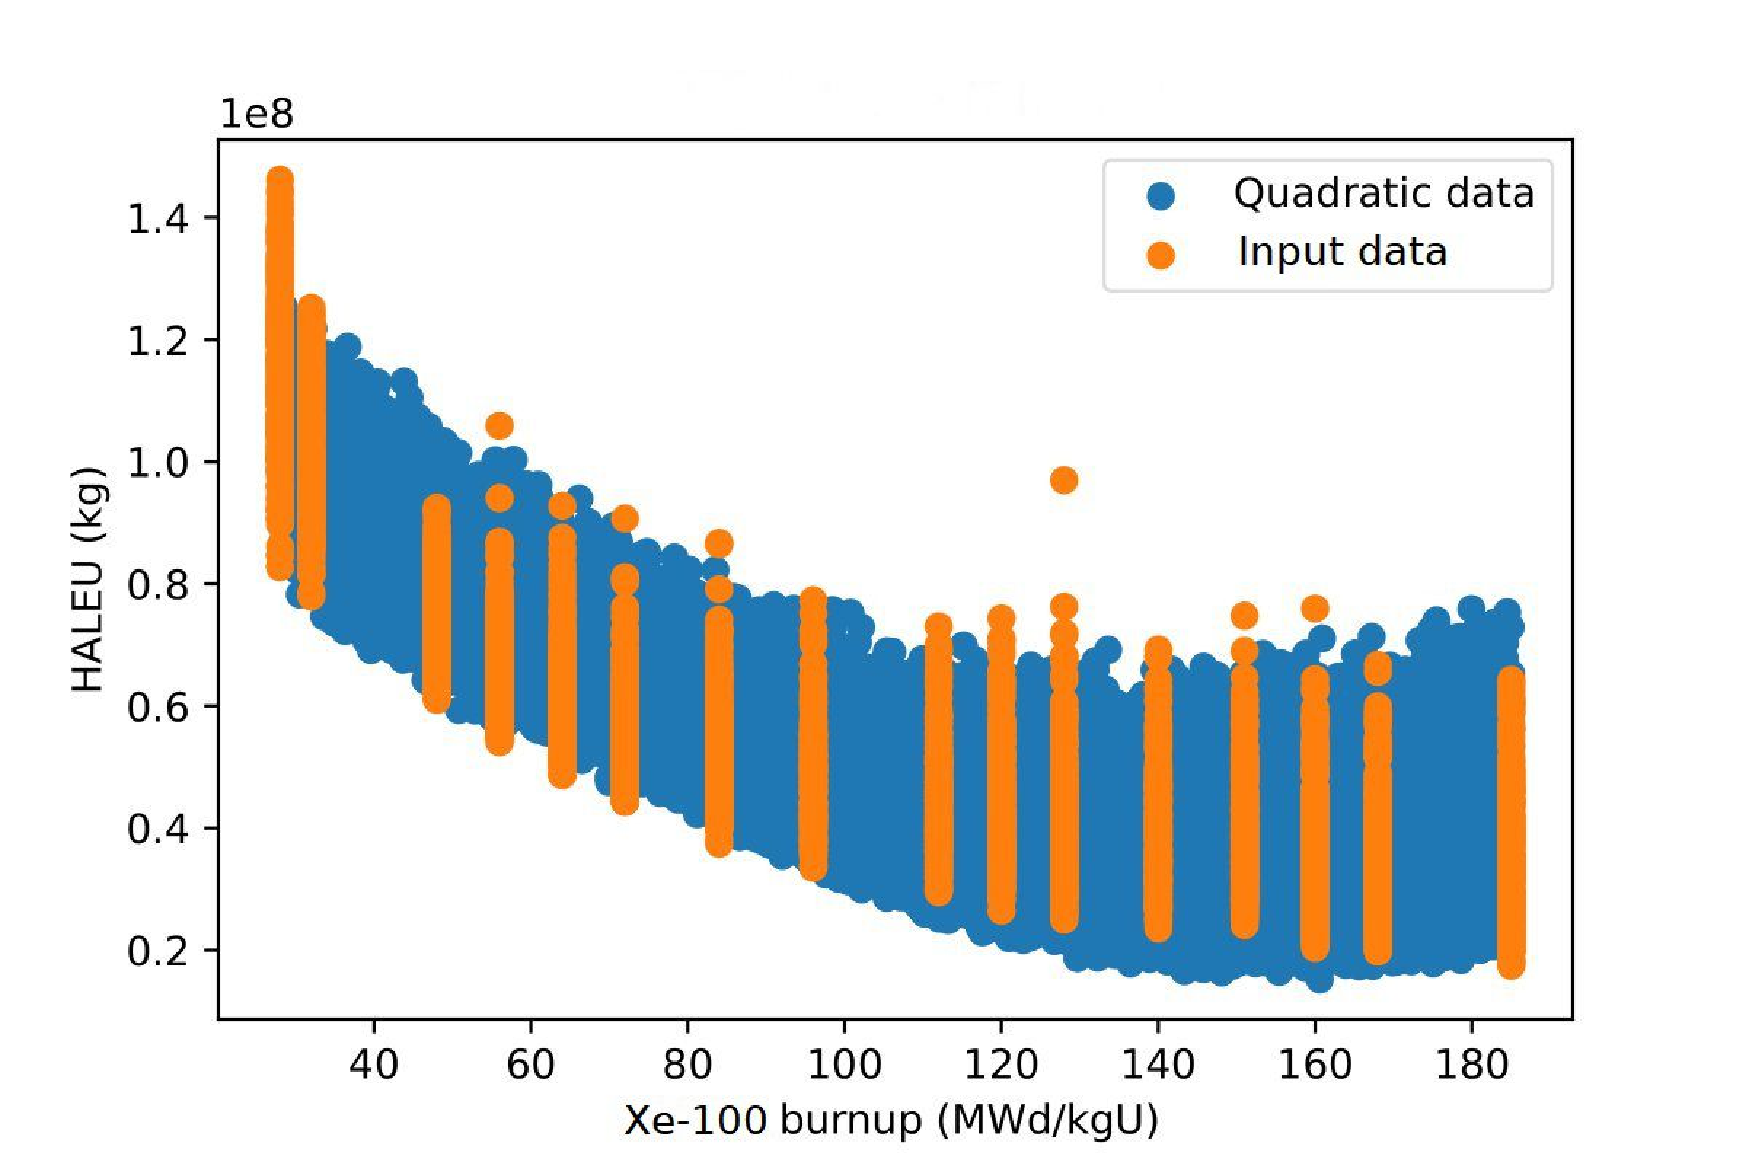
\includegraphics[scale=0.8]{mmr_share_quadratic_xe100_burnup_haleu.pdf}
    \caption{Comparison of the input data and the results of the quadratic 
    surrogate model when varying the MMR build share.}
    \label{fig:s7_mmr_quadratic}
\end{figure}

The Sobol' indices from the quadratic model (Table 
\ref{tab:s7_sobol_mmr_quadratic}) are similar to those from the 
Gaussian model. The Xe-100 burnup has the largest impact on all of the 
output metrics. The \gls{MMR} build share has the next largest impact 
on the metrics, but it is a very small impact. The other model 
parameters have a negligible effect on the metrics. The Sobol' 
indices from this model are very similar to those from the Gaussian 
model. 

\begin{table}[h!]
    \centering
    \caption{Sobol' indices for the quadratic model when varying the MMR 
    build share. The first number is the main index, the second is the total 
    index. Highlighted 
    values indicate a total Sobol' indices of above 0.5.}
    \label{tab:s7_sobol_mmr_quadratic}
    \begin{tabular}{c c c c c c c}
        \hline
        & \multicolumn{6}{c}{Output Metric} \\
        Parameter & Fuel Mass & HALEU Mass & SWU & HALEU SWU & Feed & SNF Mass \\
        \hline
        Transition Start & 0.002/0.003 & 0.000/0.000 & 0.000/0.000 &
                        0.000/0.000 & 0.000/0.000 & 0.002/0.003\\
        LWR Lifetime & 0.023/0.062 & 0.046/0.054 & 0.050/0.059 &
                       0.049/0.057 & 0.049/0.057 & 0.054/0.064\\
        MMR Build Share & 0.051/0.087 & 0.052/0.089 & 0.133/0.171 &
                          0.133/0.171 & 0.124/0.162 & 0.008/0.046\\
        Xe-100 Burnup & \cellcolor{green!25}0.834/0.866 & \cellcolor{green!25}0.846/0.875 & \cellcolor{green!25}0.742/0.764 &
        \cellcolor{green!25}0.742/0.765 & \cellcolor{green!25}0.753/0.777 & \cellcolor{green!25}0.879/0.909\\
        MMR Burnup & 0.034/0.039 & 0.034/0.040 & 0.050/0.058 & 
                     0.050/0.058 & 0.048/0.056 & 0.035/0.041\\
        \hline        
    \end{tabular}
\end{table}

\subsection{VOYGR build share}
This section provides the results of the global sensitivity analysis using 
both a Gaussian and a quadratic surrogate model when the varying the 
VOYGR build share. 

\subsubsection{Gaussian surrogate model}
The R$^2$ values for the Gaussian model with respect to 
each output metric is 1, similar to each of the other Gaussian 
models. Comparing the input data and the Gaussian model data 
(Figure \ref{fig:s7_voygr_gaussian}) shows that the data from the 
Gaussian model fits very well to the input data provided. 

\begin{figure}[h!]
    \centering 
    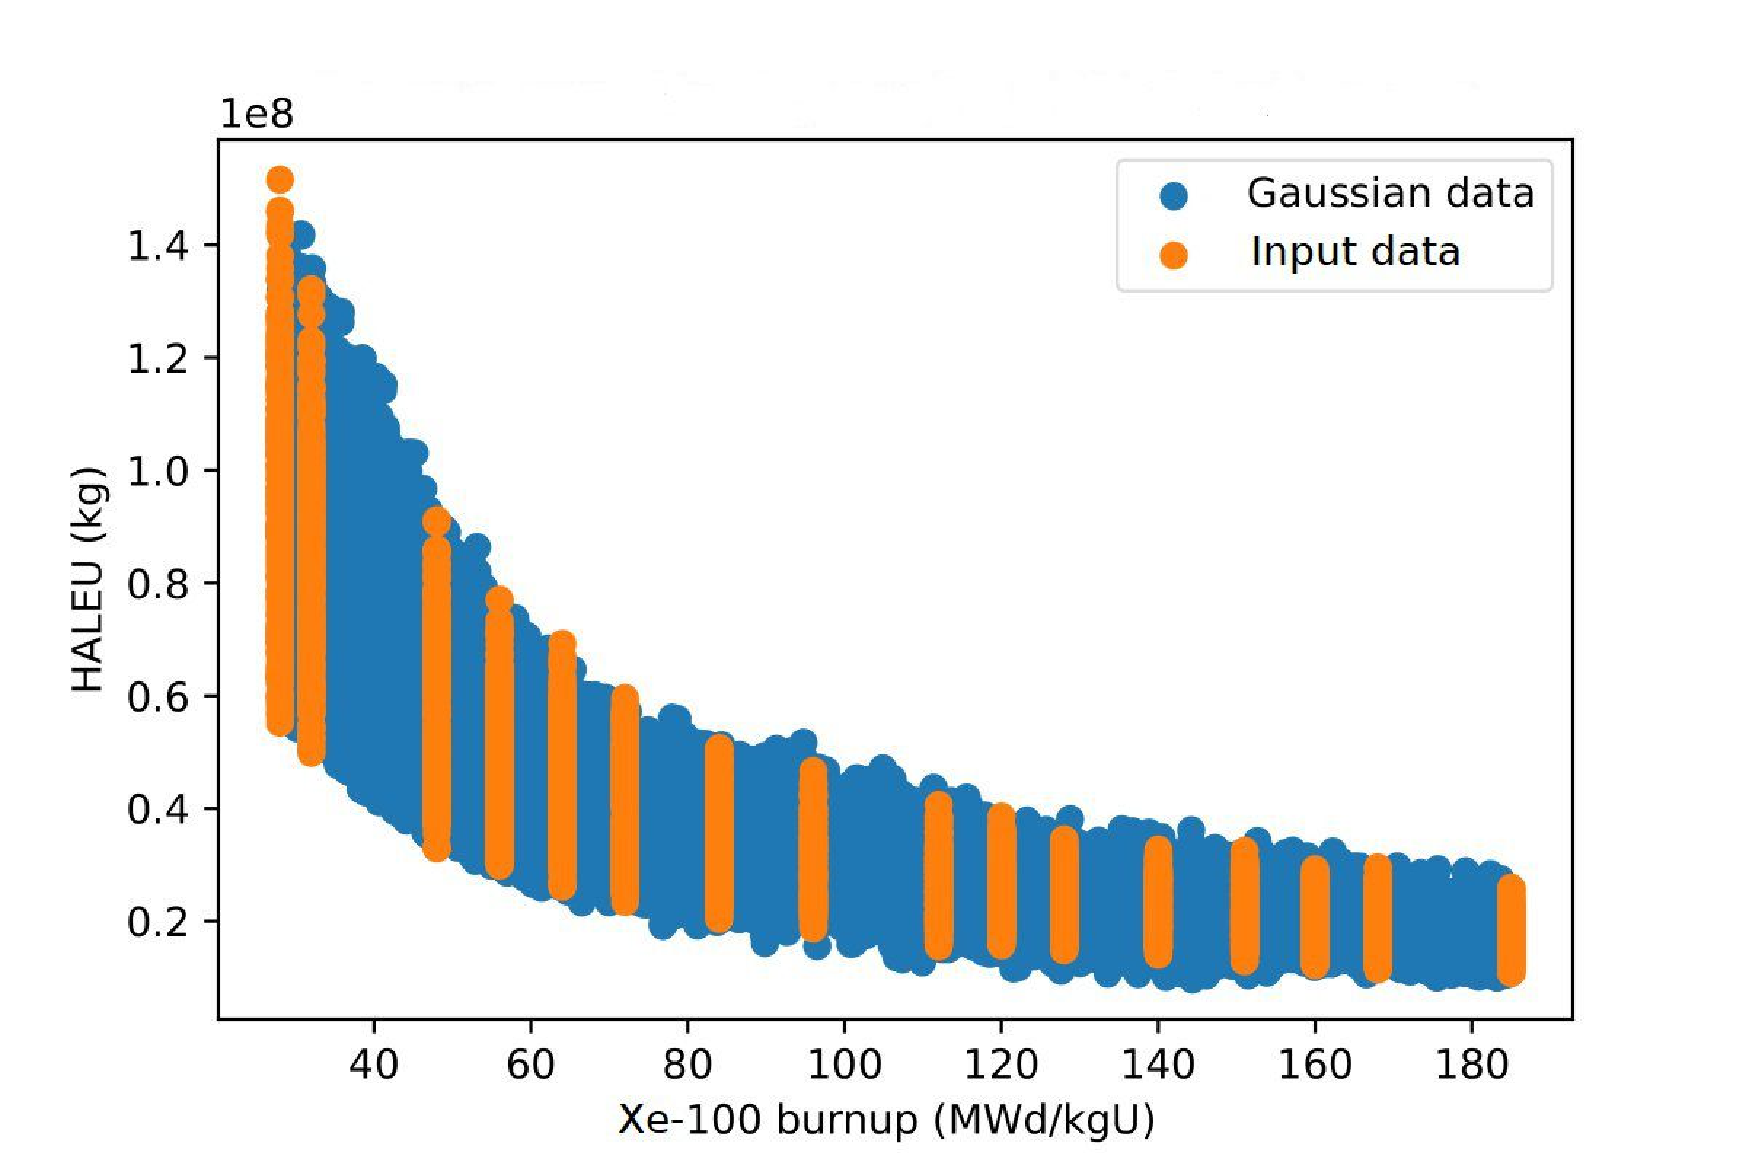
\includegraphics[scale=0.8]{voygr_share_gaussian_xe100_burnup_haleu.pdf}
    \caption{Comparison of the input data and the results of the Gaussian 
    surrogate model when the VOYGR build share is varied.}
    \label{fig:s7_voygr_gaussian}
\end{figure}

The Sobol' indices from this model, shown in Table \ref{tab:s7_sobol_voygr_gaussian}
show a similar trend to the Sobol' indices from varying the \gls{MMR}
build share. The Xe-100 burnup has the largest impact and a large impact 
(a total Sobol' indices greater than 0.5) on all of the 
results. The transition start time and \gls{MMR} burnup have effectively no 
effect on the metrics, and the \gls{LWR} lifetimes and VOYGR build share 
have a very small impact on the metrics. The \gls{LWR} lifetimes has a smaller 
effect on the metrics than when varying the Xe-100 build share, but a similar 
effect on the metrics to when varying the \gls{MMR} build share. 

\begin{table}[h!]
    \centering
    \caption{Sobol' indices for the Gaussian model when varying the VOYGR 
    build share. The first number is the main index, the second is the total 
    index. Highlighted 
    values indicate a total Sobol' indices of above 0.5.}
    \label{tab:s7_sobol_voygr_gaussian}
    \begin{tabular}{c c c c c c c}
        \hline
        & \multicolumn{6}{c}{Output Metric} \\
        Parameter & Fuel Mass & HALEU Mass & SWU & HALEU SWU & Feed & SNF Mass \\
        \hline
        Transition Start & 0.002/0.003 & 0.000/0.001 & 0.000/0.002 & 
                           0.000/0.001 & 0.000/0.001 & 0.001/0.003\\
        LWR Lifetime & 0.065/0.076 & 0.020/0.033 & 0.033/0.045 & 
                       0.020/0.033 & 0.020/0.033 & 0.069/0.081\\
        VOYGR Build Share & 0.252/0.284 & 0.114/0.0151 & 0.028/0.067 &
                            0.114/0.151 & 0.114/0.151 & 0.204/0.238\\
        Xe-100 Burnup & \cellcolor{green!25}0.652/0.683 & \cellcolor{green!25}0.837/0.883 & \cellcolor{green!25}0.910/0.956 & 
        \cellcolor{green!25}0.836/0.881 & \cellcolor{green!25}0.836/0.881 & \cellcolor{green!25}0.696/0.730\\
        MMR Burnup & 0.002/0.002 & 0.000/0.002 & 0.001/0.001 & 
                     0.001/0.002 & 0.001/0.002 & 0.002/0.002\\
        \hline        
    \end{tabular}
\end{table}

Based on the results of the \gls{OAT} analysis, increasing the VOYGR build 
share replaces 
Xe-100s with VOYGRs. Therefore, the VOYGR build share implicitly 
impacts the Xe-100 build share, which leads to this input parameter 
having a larger impact on most of the metrics than most of the other variables. 
The VOYGR build share does not have a noticeable impact on the 
total \gls{SWU} capacity because of the similar \gls{SWU} capacities 
required by the Xe-100 and VOYGR. This result is consistent with the 
Xe-100 build share having a lesser effect on this metric compared 
with its effect on the other metrics. 
The VOYGR build share has a larger impact on the fuel mass and the 
\gls{SNF} mass than the other metrics because the VOYGR takes in more 
and discharges more fuel than the Xe-100 per unit time and energy. 
The 
increased impact of the VOYGR build share on these metrics leads to 
the decreased impact of the Xe-100 burnup, relative to the 
\gls{HALEU}-related metrics. 


\subsubsection{Quadratic surrogate model}
When using the quadratic fit, the R$^2$ values range between 0.94-0.95. 
These values are consistent with the R$^2$ values for the other 
quadratic models in this work. The data from this quadratic model,
compared with the input data in Figure \ref{fig:s7_voygr_quadratic}, 
shows that it does not fully reach the maximum of the input data
and under-predicts some of the minimum values. These trends have 
been observed in all of the quadratic models created for this analysis. 
These trends are a result of the model fitting a second-order 
polynomial to data that does not follow a second order polynomial. This 
mis-fit between the data and the model fit leads to the lower R$^2$ value 
than the Gaussian surrogate models and the inability to properly fit 
to the extremes in the data. Therefore, one would expect the 
Gaussian models to be more accurate in calculating the Sobol' 
indices. The consistency between the values and trends of the 
indices from both models suggests that the quadratic models are 
still sufficient for these purposes. 

\begin{figure}[h!]
    \centering 
    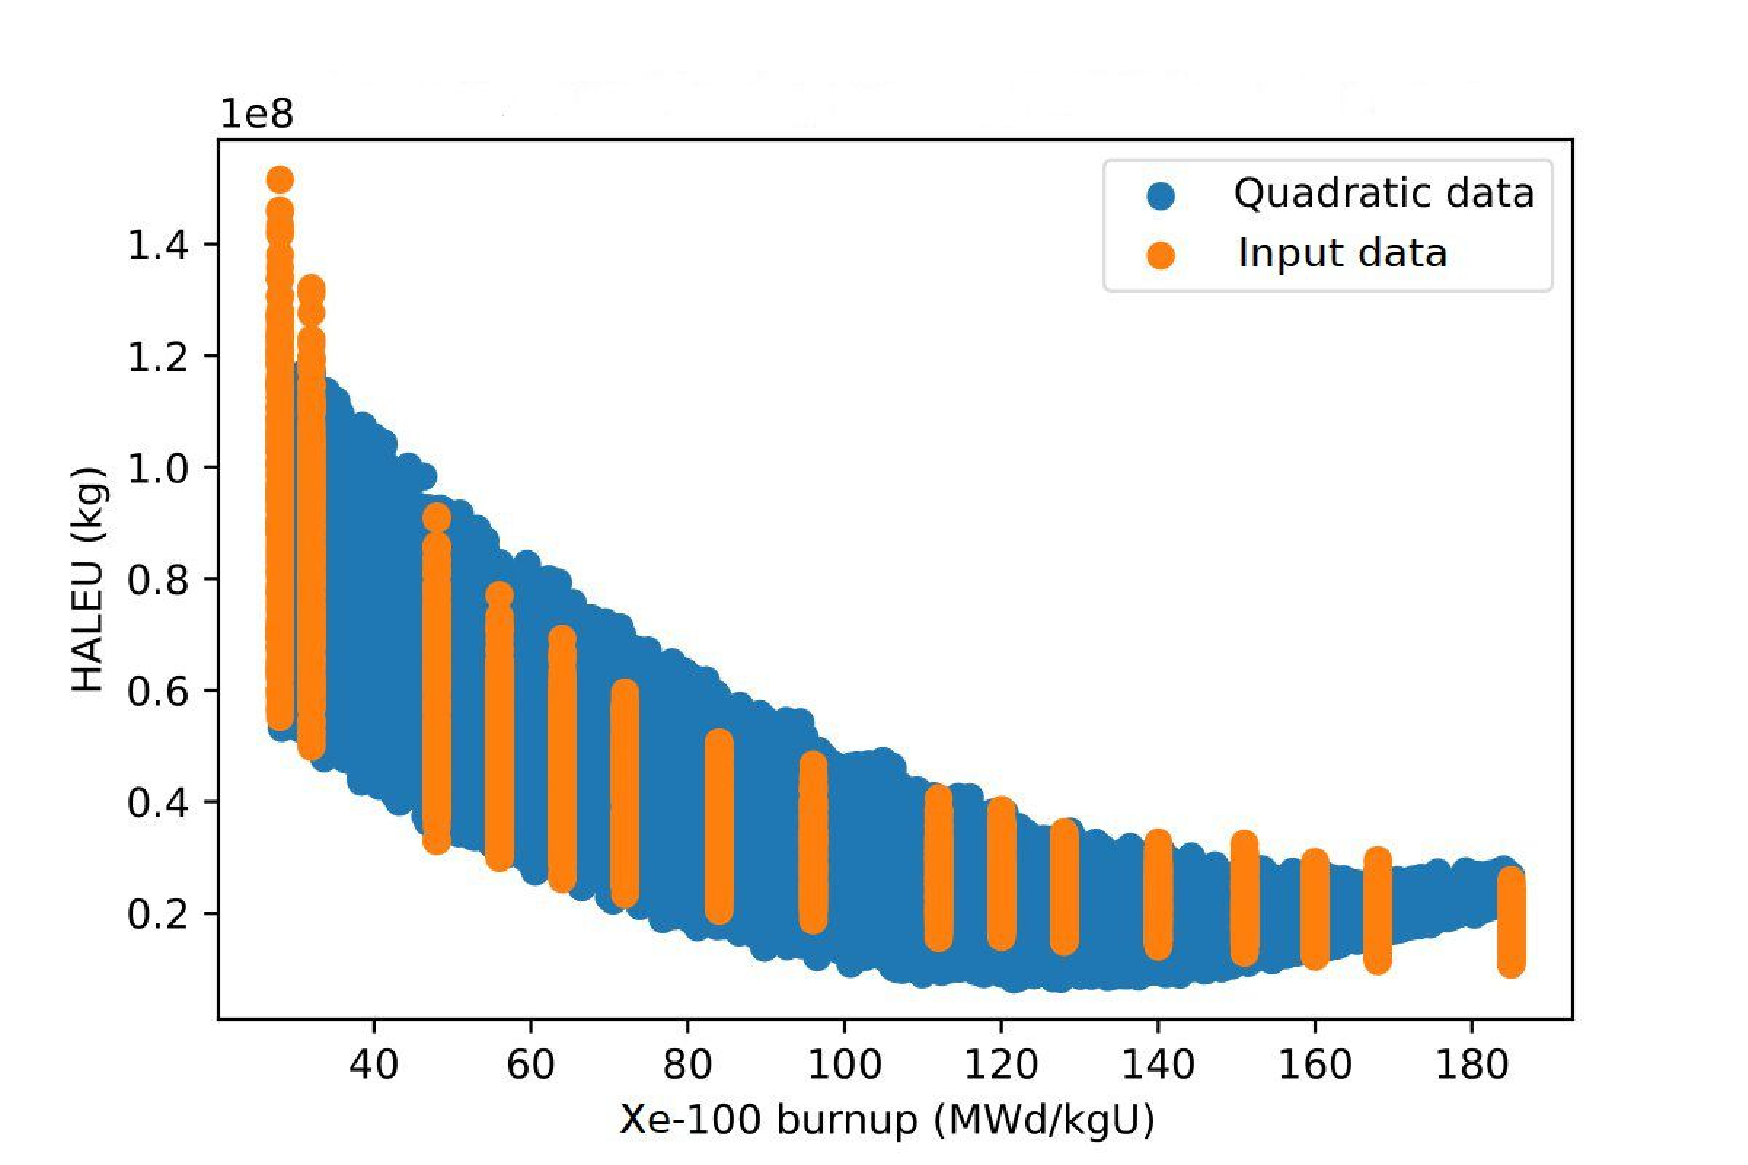
\includegraphics[scale=0.8]{voygr_share_quadratic_xe100_burnup_haleu.pdf}
    \caption{Comparison of the input data and the results of the quadratic 
    surrogate model when the VOYGR build share is varied.}
    \label{fig:s7_voygr_quadratic}
\end{figure}

The Sobol' indices from this model, reported in Table 
\ref{tab:s7_sobol_voygr_quadratic},
have the same pattern as the Sobol' indices from the Gaussian model created. 
The Xe-100 burnup is the most impactful input parameter on all of the 
output metrics, followed by the VOYGR build share and the \gls{LWR} lifetime. 
The transition start time and the \gls{MMR} burnup have a negligible effect 
on the results of the metrics. 

\begin{table}[h!]
    \centering
    \caption{Sobol' indices for the quadratic model when varying the VOYGR 
    build share. The first number is the main index, the second is the total 
    index. Highlighted 
    values indicate a total Sobol' indices of above 0.5.}
    \label{tab:s7_sobol_voygr_quadratic}
    \begin{tabular}{c c c c c c c}
        \hline
        & \multicolumn{6}{c}{Output Metric} \\
        Parameter & Fuel Mass & HALEU Mass & SWU & HALEU SWU & Feed & SNF Mass \\
        \hline
        Transition Start & 0.002/0.002 & 0.000/0.000 & 0.000/0.001 &
                           0.000/0.000 & 0.000/0.000 & 0.001/0.002\\
        LWR Lifetime & 0.063/0.071 & 0.020/0.031 & 0.031/0.042 &
                       0.051/0.031 & 0.020/0.031 & 0.066/0.075\\
        VOYGR Build Share & 0.214/0.243 & 0.108/0.143 & 0.030/0.066 &
                            0.108/0.143 & 0.108/0.143 & 0.170/0.200\\
        Xe-100 Burnup & \cellcolor{green!25}0.700/0.724 & \cellcolor{green!25}0.843/0.884 & \cellcolor{green!25}0.911/0.952 &
        \cellcolor{green!25}0.842/0.883 &\cellcolor{green!25} 0.843/0.883 & \cellcolor{green!25}0.740/0.767\\
        MMR Burnup & 0.001/0.001 & 0.001/0.001 & 0.001/0.002 &
                     0.001/0.002 & 0.001/0.001 & 0.001/0.001\\
        \hline        
    \end{tabular}
\end{table}

